\documentclass[12pt, a4paper]{report}
\usepackage{lipsum}  
\usepackage{url}
\usepackage{hyperref} 
\usepackage{float}
\usepackage{graphicx}
\graphicspath{{figures/}}

\pagenumbering{arabic}
\title{Bipedal Walking - Reinforcement Learning}
\author{Roberto Figueiredo}
\date{April 2022}


\begin{document}
\begin{titlepage}
    \maketitle 
    \thispagestyle{empty}
\end{titlepage}


\begin{abstract}
 
    This report covers the attempt to develop a bipedal walking pattern using reinforcement learning. 
 
    This project developed a series of experiments progressing from a testing ground using the CartPole environment to a 2D walker and implementation of OpenAI Gym on the RoboCup Team, Bold Hearts, ROS2 environment enabling training for any reinforcement learning task.
    The experiments cover the testing of two different learning implementations and hyperparameter tuning.
    
    
    Although the objective of walking could not be achieved in the target time frame with the limited resources available, the documentation covers the problems found along with how this difficulties were overcome. The implementation chapter will cover how each of the stages was developed, with coding examples for each of the main components.
   
    The results and findings of the experiment will be explored and an attempt to understand what could be changed to achieve achieving the desired outcome.

\end{abstract} 

\section*{Acknowledgement}
\lipsum[1-1]


\pagebreak
\tableofcontents
\pagebreak

\chapter{Introduction}
In this chapter the target problem will firstly be introduced, as will a proposed solution to solve it. To understand the problem, 
background information will be covered to better understand the problem and what it is meant to target.
% can I extend this?

\section{Introduction}
Robotic locomotion has, until a few years ago, been focused on wheel-based movement. 
Although it is very stable and easy to implement, it lacks flexibility, the ability to move on uneven, unpredictable terrain and overcome obstacles such as stairs.
\par As a RoboCup team Bold Hearts member, which competes in the humanoid soccer league, our robots must walk, a recurring problem due to rule changes. 
As the objective of RoboCup is to achieve a realistic environment, competition rules change regularly. 
Changes in rules involve field changes, such as moving from flat ground to synthetic grass, enforcing that teams develop walking algorithms that can adapt to more variable environments. 
Rule changes also affect the robots, including their height, types of sensors and others. 
Changes in the robot's structure lead to the need to readapt the walking algorithms as they are dependent on these variables. 
These changes are time-consuming, and walking algorithms are a complex task requiring much effort from the team.
\subsection{Intro to the project}

\chapter{Background Research}

    \section{Learning Algorithms}

\section{Training Framework}

\section{Previous Implementations}

\section{Logging and Reproducibility}

\chapter{Development Structure}
Due to the complexity of the project a development structure has been put in place, 
this includes multiple steps of increasing complexity and realism, 
as the increasing complexity allowed for detecting problems at an earlier, simpler stage making the transition easier.
    \section{Development Structure}
Due to the complexity of the project, a development structure has been put in place, 
this includes multiple steps of increasing complexity and realism, 
the increasing complexity allows for detecting problems at earlier, simpler stages, making the transition and understanding the problems easier.
\subsection{Cartpole}
Cartpole is a classic exercise of reinforcement learning, it consists in balancing a pole in a cart moving on an horizontal plane by applying a force on the right or left side of the cart making it move in the oposite direction. 

The cartpole environment allowes for the implementation and testing of the reinforcement learning algorithm, different implementations and its comparison, at this stage it was also used to implement the logging and reproducibility interface.

\subsection{2D Walker}
At this stage the complexity of the environment increases as the environment starts to assimilate the target problem. Although, this stage eliminates some of the complexity such as using a more complex 3D environment and implementing the training with the robot controll interface.
This allows for the implementation of a neural network, learning algorithm that is capable of handling multiple simultaneous outputs as it is required to control all the joints of the robot and understanding how to efficiently calculate the best action.

To achieve this it is necessary to develop a custom 2D environment of a simplified humanoid in order to train a walking behaviour.
New challenges from this stage such as implementing a custom reward system, rendering and step functions are an important step in order to transition to 3D simulation.

\subsection{3D Walker}
The final stage of the project is the implementation on a 3D simulated robot, this is the combination of the previous stage with extre complexity, not only due to the inherited complexity of a higher diensional world but because this should be able to integrate with the real robot from the Bold Hearts team and therefore use its control interface.
Robot simulation is the main platform for developing software for robotics, it has many benefits, developing software and testing it directly on a real robot can be a very slow process and can even lead to breaking the robot.

3d simulation brings new challenges, such as a larger range of motion and more joints to controll, along with a more complex environment, requiring more processing power and more time to solve the problem. 
Along with this it requires a more complex reward system as a new dimention poses new problems.


% values for reward goes in experiment
% what goes in the reward system goes in design


%design
%implementation
%experimental results

%author and year - reference
    \section{Environment Definition}
One of the main reasons for the use of OpenAI Gym in this project is the ability to standardize the environments.
In this section each Gym environment will be described.

\subsection{Cartpole}
The cartpole environment is a very simple exercise, consisting of a pole in a cart moving on an horizontal plane, 
the objective is to balance this pole by applying a force on the right or left side of the cart making it move in the oposite direction.
\cite{cartpole}

\begin{figure}[H]
    \centering
    \includegraphics[scale=0.24]{cartpole}
    \caption{Rendered Cartpole Environment - OpenAI Gym}
\end{figure}

Cartpole Environment definition:
\begin{itemize}
    \item \textbf{Observation Space}
            \begin{table}[H]
                \caption{Observation Space for the Cartpole environment}
                \centering
                \begin{tabular}{|l|l|l|l|}
                \hline
                Num & Observation           & Min  & Max  \\ \hline
                0   & Cart Position         & -4.8 & +4.8 \\ \hline
                1   & Cart Velocity         & -Inf & +Inf \\ \hline
                2   & Pole Angle            & -24° & +24° \\ \hline
                3   & Pole Angular Velocity & -Inf & +Inf \\ \hline
                \end{tabular}
                \end{table}
    \item \textbf{Action Space} 
    \begin{table}[H]
        \caption{Action Space for the Cartpole environment}
        \centering
        \begin{tabular}{|l|l|}
        \hline
        Num & Action                 \\ \hline
        0   & Push cart to the left  \\ \hline
        1   & Push cart to the right \\ \hline
        \end{tabular}
        \end{table}
    \item \textbf{Reward:} In the cartpole environment the reward is attributed per timestep survived, being awarded 1 point per timestep.
    \end{itemize} 

\subsection{2D Walker}
The 2D environment requires a 2D Humanoid, this has been defined with 8 different joints, 2 in the shoulder, 2 in the hips, 2 in the knees and 2 for the ankles.
\begin{figure}[H]
    \centering
    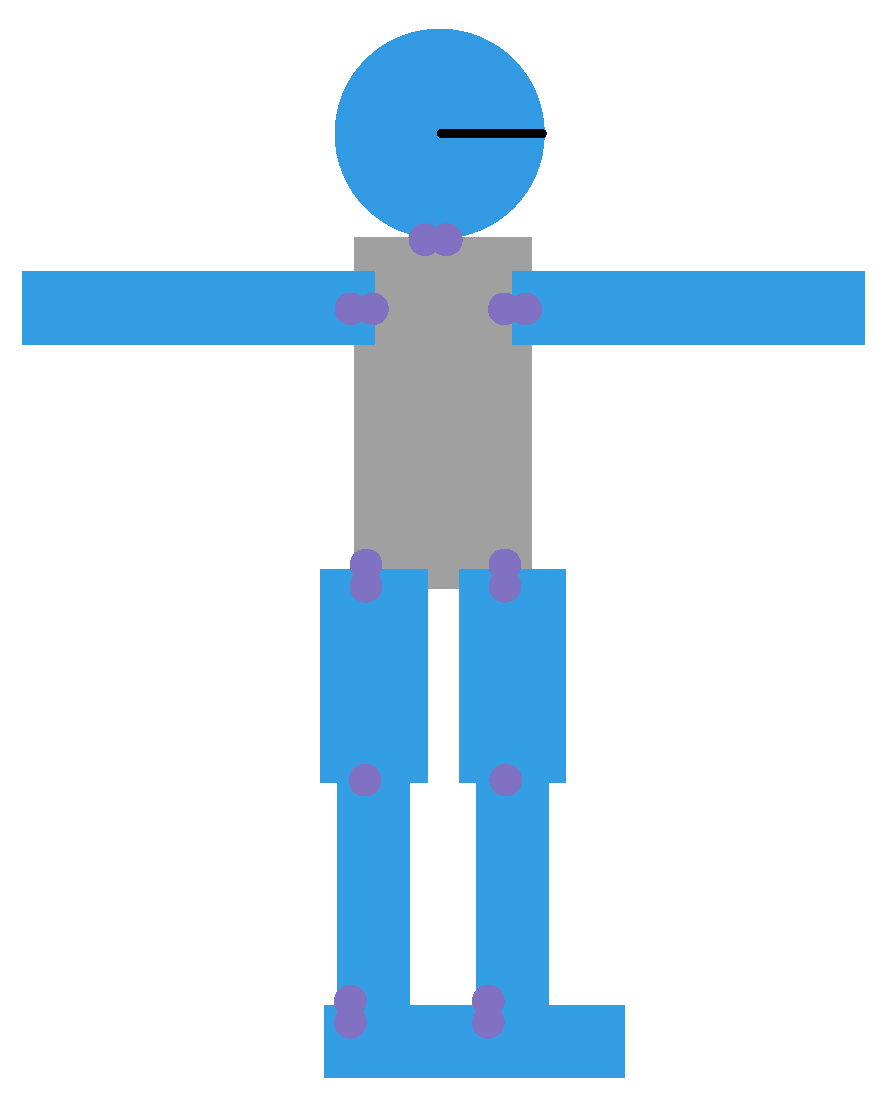
\includegraphics[scale=0.25]{humanoid-2d}
    \caption{Representation of 2D humanoid}
\end{figure}

Environment definition:
\begin{itemize}
    \item \textbf{Observation Space:} The Observation Space is a vector of size 8, containing the angles for each of the 8 joints of the humanoid.
    \begin{table}[H]
        \caption{Observation Space for the 2D Walker environment}
        \centering
        \begin{tabular}{|l|l|l|}
        \hline
        Observation           & Min  & Max  \\ \hline
        Joint Position         & -20° & +20° \\ \hline

        \end{tabular}
        \end{table}

    \item \textbf{Action Space:} 
    \begin{table}[H]
        \caption{Action Space for the 2D Walker environment}
        \centering
        \begin{tabular}{|l|l|}
        \hline
        Num & Action                 \\ \hline
        0   & Move the joint counterclockwise  \\ \hline
        1   & Maintain joint position \\ \hline
        2   & Move the joint clockwise \\ \hline
        \end{tabular}
        \end{table}
    \item \textbf{Reward:} 
    \begin{table}[H]
        \caption{Reward system for the 2D Walker environment}
        \centering
        \begin{tabular}{|l|l|}
        \hline
        Action & Points                 \\ \hline
        Moves Back   &  - 2  \\ \hline
        Stays in Place   & -1 \\ \hline
        Moves Forward   & 1 \\ \hline
        Loses contact with the ground & cumulative -2 \\ \hline
        Reaches target & 10 \\ \hline
        Falls & -10 \\ \hline
        \end{tabular}
        \end{table}
    
\end{itemize}

\subsection{3D Walker}
In the 3D environment, the robot needs to simulate the one used by the Bold Hearts team, given that the team already uses a simulator, gazebo, this will be used to interact with the robot given that it provides ROS2 integration.
\begin{figure}[H]
    \centering
    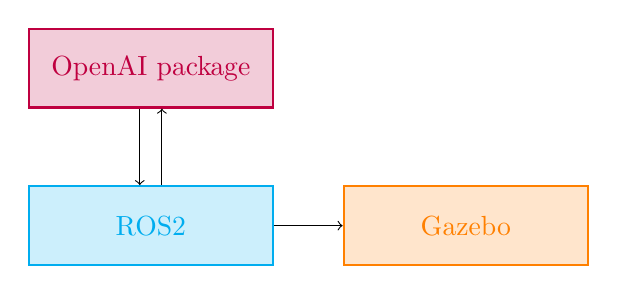
\begin{tikzpicture}[every node/.style=draw]
        \node[rectangle, 
        draw, 
        thick,
        minimum width = 3.1cm,
        minimum height = 1cm,
        color=cyan,
        fill=cyan!20] (A) at (0,0) {ROS2};
        \node[rectangle, 
        draw, 
        thick,
        minimum width = 3.1cm,
        minimum height = 1cm,
        color=purple,
        fill=purple!20] (B) at (0,2) {OpenAI package};
        \node[rectangle, 
        draw, 
        thick,
        minimum width = 3.1cm,
        minimum height = 1cm,
        color=orange,
        fill=orange!20] (C) at (4,0) {Gazebo};

        \draw [->] ([xshift=-4]B.south) to  node [midway,left, draw=none]{} ([xshift=-4]A.north);
        \draw [<-] ([xshift=4]B.south) to  node [midway,left, draw=none]{} ([xshift=4]A.north);
        \draw [->] (A.east) to  node [midway,left, draw=none]{} (C.west);
    
    \end{tikzpicture}
    \caption{Integration of ROS2, Gazebo and OpenAI Gym}
\end{figure}

To achieve this integration, OpenAI Gym should be able to subscribe ROS2 topics containing the world observations. 
The OpenAI Gym should also be able to publish to ROS2 topics, allowing it to control the robot's joints, as well as calling services in order to controll the simulation, including, pause and reset the simulation.
One of the main aspects of this integration is to allow to train not only walking but also any relevant task by the team, to achieve this the OpenAI Gym package should be split into three different parts:
\begin{itemize}
    \item Robot
    \item Environment
    \item Task
\end{itemize}
The robot file should contain all the setup required for the Boldbot, the teams robot. On the Environment file all the environment setup should be defined, such as the observation space, action space, reward system, etc. 
Finaly the task file should be specific for the task trying to be achieved, allowing the team to setup just the task without requiring setting up the robot and environment everytime.
\cite{ros-gym} % TODO: expand on the specific files

%TODO: Add the reward system, actions and observation space if possible


\chapter{Results}
    
\section{Cartpole Outcomes}
The first task developed was the classic cartpole environment,
this was helpfull in understanding core concepts of reinforcement learning and neural networks, along with it,
cartpole was essential in testing and setting up the logging interface as well as testing different implementations of the learning algorithm 
\subsection*{Keras-rl}
Keras-rl is a community maintained high level implementation of keras agents for reinforcement learning, this was the first implementaiton tested. 



The implementation of keras-rl is very easy and diesn't require a deep understanding of reinforcement learning and the leanring structure.
\subsection*{Keras API}
The second implementaiton tested was using the plain keras API, while this provides more flexibility it also requires a much deeper understandng of how reinforcement learning works.
%%%%%%%%% INSERT DETAILS HERE %%%%%%%%%
The implementaiton using the Keras API was essential to develop a necessary knowledge for the project and to progress to the next stage.
\subsection*{}

While an implementaiton using Keras-rl would be simpler and even possibly ease the itteration process, this implementation provides less flexibility and given the target of the project and 
desire to develop a deeper understanding of reinforcement learning the implementation using the Keras API was choosen to implemnt the next phases.

\subsection*{Results}

%%%%%%%%% INSERT RESULTS DATA AND ANALYSIS HERE %%%%%%%%%%%%%%%%%%

\section{2D Environment Outcomes}

\section{3D Environment Outcomes}

\section{Reward Function}



\chapter{Future Research}
    \chapter{Future Research}
Reinforcement learning is a very complex topic, specifically when applied to such a complex movement as robotic bipedal walking. There are many approaches to solving reinforcement learning problems. Although many areas of interest couldn't be covered, this can be explored in future research on Bipedal Robotic walking and reinforcement learning in general.

As was shown in this report, developing an optimal reward function can be complex, which is an unsolved problem in the reinforcement learning field. One promising topic suggested by the project supervisor was empowerment\cite{empowerment} by intrinsic motivations. Empowerment is a technique that aims to overcome the reward problem by equipping the robot with intrinsic rewards, using rewards such as curiosity and empowerment.

The developed project uses discrete actions although, there is a loss of information when using this method, for future research, it would be valuable to compare a policy gradient approach using continuous actions.

The initial design for this project was to use Mujoco as a physics engine. However, due to time constraints, the plan had to be changed to use Gazebo as the environment was already modelled and integrated directly with ROS2. Nonetheless, the use of Mujoco is still of interest to the team, and a comparison against Gazebo can be researched.

One of the problems when developing something as simple as a motion script for the robot is the transition to the real robot, while the script might work perfectly in the simulator, it will require adaptation to work on the real robot. This is a topic of interest for the future and understanding how, using the simulator to train most of the movement, the learning can be transferred to the real robot and how to tune the learned model when testing on the robot.



\chapter{Project Evaluation}
    \chapter{Project Evaluation}
Walking for bipedal robots using reinforcement learning was an ambitious project. Although walking could not be achieved, this project successfully developed a working 2D walking environment with a simple humanoid, implementing OpenAI Gym with ROS2 and developing documentation and preparation for future research on the topic.

The training for this project was mainly executed using Google colab+, as incompatibilities with the computer architecture (ARM64) made training locally slower in comparison. Although, Google colab constantly crashed due to timeouts and unknown problems, making it impossible to train for extended periods of time. 
On a retrospective, it would have been a better decision to train locally as even if the training was slower, it would be able to run for very long periods of time.

As already explored, the reward function should have been tested from the beginning exclusively with positive rewards, as this would have allowed for a more efficient experiment.



Although no training was executed, the last stage was a significant achievement as it is a useful tool and development not exclusive to this project but for the team. 

\chapter{Conclusion}
    \include{MainContent/conclusion.tex}
\bibliographystyle{plain}
\bibliography{reference}
\end{document}

